\newpage
\section{File I/O}


% Introduzione
\subsection{Chiamata open}

I file I/O sono le \hl{funzioni che gestisce buffered I/O} ed in contrapposizione da quelle della libreria "stdlib". La chiamata open() fa parte di queste funzioni, i suoi argomenti sono:

\begin{itemize}
	\item \hl{arg}: path assoluto o relativo
	\item \hl{flag}: bit che indica l'\textbf{attivazione di alcune modalita'}. Si avrà allora a \textbf{settare il bit della flag a 1}:
	\item \hl{mode}: serve a dare i \textbf{privilegi con cui i file deve essere creato} (\textbf{da usare solo nella creazione del file})
\begin{lstlisting}
open(file, O_RDWR | O_APPEND | O_CREAT | O_TRUNC, file_mode)
\end{lstlisting}

		avremo allora $11000001010$ con:
		
		\begin{itemize}
			\item[] O\_RDWR = 2
			\item[] O\_APPEND = 8
			\item[] O\_CREAT = 512
			\item[] O\_TRUNC = 1024
		\end{itemize}
		
\end{itemize}


% Read e write flag
\subsection{Read e write flag}

I \hl{bit delle flag} abbiamo un modo "scomodo" per rappresentarle dato che non seguono la normale "accensione dei singoli bit":

\begin{lstlisting}
#define O_RDONLY   0x0000 /* reading only */
#define O_WRONLY   0x0001 /* writing only */
#define O_RDWR     0x0002 /* reading and writing */
#define O_ACCMODE  0x0003 /* above modes */
\end{lstlisting}

sono dette \hl{maschere} per leggere o scrivere.


% Chiamata openat()
\subsection{Chiamata openat()}

\hl{Prende un file descriptor} (passato dalla open() sulla directory) di una directory per passare il path relativo a quella directory. La sua \hl{falla nel sistema} sta nella possibilità di \hl{continuare ad accedere a file anche dopo che sono cambiati i privilegi}, dato che lasciando aperta la sessione del file non saremo soggetti ai nuovi privilegi.

Questa chiamata è \hl{interessante per le Thread} che vogliono lavorare in un loro ambiente.


% Open flags
\subsection{Open flags}

Abbiamo un certo numero di \hl{flag standard} dichiarate dall'SUSv3, il resto possono essere a discrezione dei sistemi UNIX.

Le flags più usate sono:

\begin{itemize}
	\item \hl{O\_DIRECTORY}: \textbf{limita la chiamata} open ad una directory specifica

	\item \hl{O\_CREAT}: flag per dire che si vuole \textbf{creare un file}

	\item \hl{O\_TRUNC}: se vuoi creare un file nuovo ed ne esiste già uno, il \textbf{vecchio viene azzerato}

	\item \hl{O\_EXCL}: se il file già esiste fa \textbf{fallire la chiamata}
\end{itemize}


% Builtin umask
\subsection{Builtin umask}

È un \hl{valore presente in ogni processo} ed ereditato dal parent ma il child può comunque modificarla. Il valore restituito è un numero ottale (inizia con 0):

\begin{lstlisting}
$ umask
0022

$ ll file
-rw-r--r-- 1 docente staff 0 14 Ott 09:02 file
\end{lstlisting}

quindi la umask \hl{taglia i permessi dei file creati da quel processo}. Quindi, in questo caso, un 666 diventa 644.


% Chiamata lseek()
\subsection{Chiamata lseek()}

Per un file appena creato la sua "current position" si trova all'inizio del file, ci si \hl{potra' muovere nel file} tramite lseek(). Gli argomenti sono:

\begin{enumerate}
	\item \hl{file descriptor}
	
	\item \hl{offset}: per dire \textbf{dove ci si vuole spostare}
	
	\item \hl{whence}: indica \textbf{da quale punto} si deve applicare l'offset:
	
		\begin{itemize}
			\item SEEK\_SET: valore preciso da dove partire
			
			\item SEEK\_CUR: presa la current position inserire un \textbf{gap e poi scrivere} (può essere negativo)
			
			\item SEEK\_END: gap dal quale inserire \textbf{rispetto alla fine} del file. Se negativo scrivo prima, se positivo posso lasciare un \textbf{buco di byte} e poi scrivere. Nei nuovi sistemi i blocchi vuoti vengono allocati.
		\end{itemize}
	
	
\end{enumerate}

Un esempio di buco in un file dato da un numero positivo con SEEK\_END:

\begin{lstlisting}
#include "apue.h"
#include <fcntl.h>

char	buf1[] = "abcdefgh";
char	buf2[] = "ABCDEFGH";

int
main(void)
{
	int		fd;

	if ((fd = creat("file.hole", FILE_MODE)) < 0)
		err_sys("creat error");

	if (write(fd, buf1, 10) != 10)
		err_sys("buf1 write error");
	/* offset now = 10 */

	if (lseek(fd, 16384, SEEK_SET) == -1)
		err_sys("lseek error");
	/* offset now = 16384 */

	if (write(fd, buf2, 10) != 10)
		err_sys("buf2 write error");
	/* offset now = 16394 */

	exit(0);
}	
\end{lstlisting}

avremo:

\begin{lstlisting}
$ xxd file.hole
00000000: 6162 6364 6566 0000    abcdefgh........
00000010: 0000 0000 0000 0000    ................
00000020: 0000 0000 0000 0000    ................
00000030: 0000 0000 0000 0000    ................
00000040: 0000 0000 0000 0000    ................
00000050: 0000 0000 0000 0000    ................
00000060: 0000 0000 0000 0000    ................
00000070: 4142 4344 4546 4748    ABCDEFGH........
\end{lstlisting}

abbiamo che la memoria sul disco è:

\begin{lstlisting}
$ du -h file.hole 
1.6M	file.hole
\end{lstlisting}

invece la size del file è:

\begin{lstlisting}
$ stat -x file.hole 
  File: "file.hole"
  Size: 1638410      FileType: Regular File
  Mode: (0644/-rw-r--r--)         Uid: (  501/    matt)  Gid: (   20/   staff)
Device: 1,16   Inode: 27657406    Links: 1
Access: Fri Oct 14 09:59:17 2022
Modify: Fri Oct 14 09:57:59 2022
Change: Fri Oct 14 09:57:59 2022
 Birth: Fri Oct 14 09:47:24 2022
\end{lstlisting}

Possiamo avere dei \hl{file descriptor seekble} se il file è regolare o meno:

\begin{lstlisting}
#include "apue.h"

int
main(void)
{
	if (lseek(STDIN_FILENO, 0, SEEK_CUR) == -1)
		printf("cannot seek\n");
	else
		printf("seek OK\n");
	exit(0);
}
\end{lstlisting}








ci sono più casi in cui il numero di byte letto è minore di quello chiesto:
1. possiamo avere un valore di ritorno di 50 se chiedo di leggere 100 perchè ci sono solo 50 byte
2. quando legge da un terminale: la read ritorna quando dai invio
3. quando legge da una rete: puoi leggere 100 byte ma se ne leggi 10 puoi gestire tu cosa fare, in genere se non arriva nulla la read rimane in attesa e non gli arrivano byte rimane appesa sennò se sono arrivati rimane appesa e poi interrompe quando non sente più nulla
4. quando legge da una pipe: se non arriva nulla rimane appesa, se arriva qualcosa interrompe e restituisce quello che ha letto
5. quando interrotta da un segnale e alcuni dati sono stati letti gli restituisce








i/o effitiency:

\begin{figure}[H]
\centering
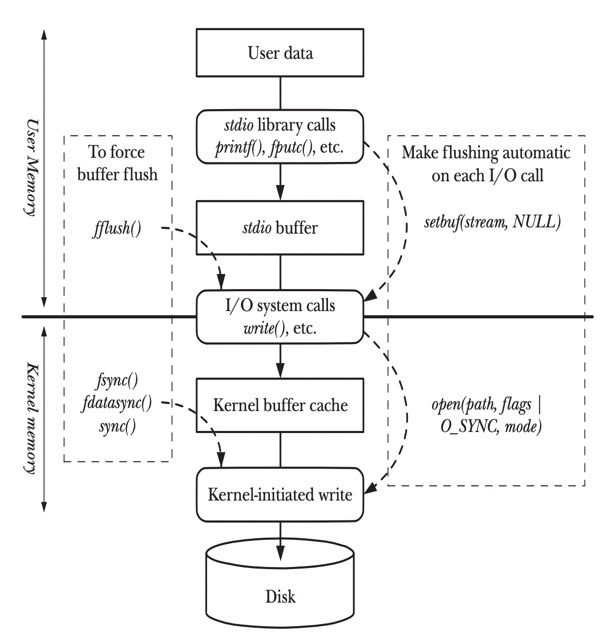
\includegraphics[scale=0.4]{unbuffio.jpeg}
\caption{Schema unbuffered I/O} 
\label{unbuffio}
\end{figure}

se devo tranferier una grande quanità di dati e la write ha un buffer limitato quanto posso mandare alla volta? ci sara1 una dimensione ottimale da trovare. i tempi possono essere misurati con time per capire in nostro giga di byte in che modo debba essere sezionato se in K o M ecc fino ad ottenere un valore ottimale.

(provare a fare ciò tramite intro/mycat e tramite time capire le tempistiche (A CASA))








file shaing:

noi abbiamo un file e potrebbero essere ci più processi che se lo contengono tra di loro per poterci accedere.


img 3.7


abbiamo una process table entry con i vari file descriptor con il loro flag ed il puntatore ala memoria delle file table entry.Ogni file dscriptor avrà una file table entry, quidni ci saranno tanti file table quanti fd ci sono. le quali hanno:

\begin{itemize}
	\item file status flags: 
	\item current file offset: 
	\item v-node pointer: (con v=virtual) puntatore ad una v-node table entry che contiene i dati, cioè:
		\begin{itemize}
			\item v-node information
			\item v\_data: puntatore all'inode
		\end{itemize}
\end{itemize}


ora vediamo un caso con più processi che puntano allo stesso file:


img 3.8


ogniuno ci arriva con un suo file offset e flags. se 2 processi si mettono a scrivere insieme servirà qualcuno che gestisce il tutto altrimenti ci sarà un override della scrittura del secondo sul primo.







per fare un'append senza avere il flag O\_APPEND, allora usiamo la funzione lseek() per mettersi alla fine del file e poi scrivere.

dato che abbiamo lseek che ancora non ha scritto e qualcun'altro chiama lseek avremo una sovrascirtzzion. il kernel mentre fa questa cosa fa solo quella e non permette a un altra systemcall di intromettersi in modo da avere delle operazioni atomiche. questo lo gestisce il porgrammatore del kernel.O\_APPEND fa diventare atomica lseek e write.

esistono delle chiamate che fanno cio1 che fa O\_APPEND ma se 2 processi vogliano scrive nello stesso file esistoon 2 chiamata per fare lseek e write insieme:

pwrite(): identica ala write ma ha un paramentri di offset quindi di effettua un'operazione atomica andando a scriere proprio in quel punto senza rischio che le operazione di spostarsi e scrivere non si pestino i piedi tra loro. se 2 processi vogliono srivere nello stesso punto si sposta il primo in un punto e srive tutto nel pochi millisencondi per poter fare entrambe le system call rendendo il tutto atomico.

altra operazione atomica: creazione di un file con flag O\_EXCL. in questo caso ci sono dei problemi: se un prcesso vuole aprire un file in modo esclusivo, se esite non lo crea ma possono scedre particci dato che se il file non ci fosse il sistema ti dice che puoio creare il file ma nello stesso momento un altro porcesso va a crearlo allora tu vai a sovrascrivere. usanto queti flag si fara1 creazioene e scrittura del file nello stesso momento rendendo l'operaizone atomica.

se c'e1 la necessità che due file non si pestino i piedi allora un pircesso crea in modo esclisivo un file facendo le operazioni che deve fare, l'altro processo ricevera1 un errore daro che il file esiste. alla il primo potrà eliminare il file in modo da potrlo far scrivere dal primo qundo riproverà. questo serve per effettuare una sincronizzazione. quidni il primo porcesso scrive quello che deve in un file e v=crea quello "farlocco" per potersi prenotare il nome del file. 





2 funzioni:

up: prende un file descriptor e restituisce un numero che e1 un duplicato di quel fd. quidi abbiamo 2 fd che puntano alla stedda file table.


img 3.9


dup2: prende un fd da duplicare dicendogli anche il numero del fd. ma se il numero che gli passiamo è già preso allora sifoza la chiusura del fd e lo si assegna a ciò che vogliamo.



vediamo cosa succede in questo ambito con fork e child:


img 8.2 


dopo una fork i processi child e parent sono uno la copia dell'altro quindi avremo che i fd del child punteranno alle stesse file table e quindi agli stessi spazi di memoria alla quale accedono entrambi. Abbiamo quindi il problema che se il child modifica qualcosa lo vedrà anche il parent





ridirezzione ad un file:

quindi abbiamo che quando apriamo un file civiende dato un fd 3, se favvio una dup2(3, 1) abbiamo la ridirezione a file. a fare tutte queste operazioni è lo shell e grazie alla eredità fd i processi dopo la fork avranno già tutti i dati.

avremo a gestire questo il flag CLOEXEC: quanto lo shell vede la ridirezione ($>$) allora dice che se sei il child fai un'apertura del file ed ottiene fd 3 allora da una dup(3, 1) poi fa una exec e se il flag è 0 (cioè non chiudere quando fai un exec) allora il processo successivo avrà in input l'output del precedente  processo

invece è ad 1 il flag quando vogliamo che il fd venga chiuso nel prossimo processo e quindi potrà essere usato come fd più basso da attribuire


funzione fcntl:
 effettua controlli sul fd. è un coltellino svizzero dat che ha come paramentri fd, cmd e altri dove cmd è usto per dichiamare delle funzionalità specifiche:

- F\_DUPFD: si duplica il fd. tramite il terzo argomento avremo all'assegnazione di un fd $\geq$ del valore di quell'argomento

- F\_GETFD, F\_SETFD: get/set fd flag

- F\_GETFL, F\_SETFL: get/set file status flag (per cambiare il flag mentre il file è ancora aperto)

- F\_GETLK, F\_SETLK: get/set record locks: servono a bloccare parti di file


notiamo l'apertura diversa dei fiel tramite:

\begin{lstlisting}
#include "apue.h"
#include <fcntl.h>

int
main(int argc, char *argv[])
{
	int		val;

	if (argc != 2)
		err_quit("usage: a.out <descriptor#>");

	if ((val = fcntl(atoi(argv[1]), F_GETFL, 0)) < 0)
		err_sys("fcntl error for fd %d", atoi(argv[1]));

	switch (val & O_ACCMODE) {
	case O_RDONLY:
		printf("read only");
		break;

	case O_WRONLY:
		printf("write only");
		break;

	case O_RDWR:
		printf("read write");
		break;

	default:
		err_dump("unknown access mode");
	}

	if (val & O_APPEND)
		printf(", append");
	if (val & O_NONBLOCK)
		printf(", nonblocking");
	if (val & O_SYNC)
		printf(", synchronous writes");

#if !defined(_POSIX_C_SOURCE) && defined(O_FSYNC) && (O_FSYNC != O_SYNC)
	if (val & O_FSYNC)
		printf(", synchronous writes");
#endif

	putchar('\n');
	exit(0);
}	
\end{lstlisting}

infatti abbiamo:

\begin{lstlisting}
$ ./fileflags 0 < /dev/ttys000
read only

$ ./fileflags 1 > prova.txt
$ cat prova.txt 
write only

$ ./fileflags 2 2>>prova.txt 
write only, append

$ ./fileflags 5 5<>prova.txt 
read write
\end{lstlisting}

per inserire o togliere i flag usiamo:

\begin{lstlisting}
val |= flags;		/* turn on flags */
val &= ~flag;		/* turn off flags */
\end{lstlisting}





sappiamo che unix vedo tutto come un file con le sue funzion open read write close. la funzione ioctl() è detta catchall per operazioni I/O.





CAP 4:

funzione stat: legge l'inode e ti dice le cose che puoi sapere riferite all'inode. tramite il comando dumpe2fs ceh fa il dump di tutta la struttura dati nella patizione disignata. dove abiamo la desrizione del file system.

se vogliamo trovare i puntatori ed i blocchi di un file dato il suo nome andiamo a guardare l'inode del file e poi atrovare i blocchi. tramite il comando dd posisamo andare tagliare i blocchi nel file che rappresenat la nostra partizione dove ci saranno da rispettare alcune regole sul qualti byte rappresentano un blocco ecc (regole del file system) 

stat prendere:

\begin{lstlisting}
int stat(const char *restrict pathname, struct stat *restrict buf);
\end{lstlisting}

- path: del quale dire i dati
- struct: parametri di uscita dato che è un puntatore

abbiamo delle varianti:
fstat: usa un fd al posto del path
lstat: prende dei link simbolici in pathname (può esser usata anche per file normali)
fstatat: prende sia un fd che un pathname


nella struttura stat abbiamo tutti i dati che abiamo come output dalla funzione:

\begin{lstlisting}
struct stat {
	mode_t		st_mode;		/* file type & mode (permissions) */
	ino_t		st_ino;			/* i-node number (serial number) */
	dev_t		st_dev;			/* device number (file system) */
	dev_t		st_rdev;		/* device number for special files */
	nlink_t		st_nlink;		/* number of links */
	uid_t		st_uid;			/* user ID of owner */
	gid_t		st_gid;			/* group ID of owner */
	off_t		st_size;		/* size in bytes, for regular files */
	struct timespec st_atim;	/* time of last access */
	struct timespec st_mtim;	/* time of last modification */
	struct timespec st_ctim;	/* time of last file status change */
	blksize_t	st_blksize;		/* best I/O block size */
	blkcnt_t	st_blocks;		/* number of disk blocks allocated */
};
\end{lstlisting}